\documentclass[14pt]{article}
\usepackage[utf8]{inputenc}
\usepackage[T2A]{fontenc}
\usepackage[russian]{babel} % Кириллица uchun, lekin matn lotin yozuvida
\usepackage{amsmath, amssymb}
\usepackage{geometry}
\usepackage{graphicx}
\usepackage{xcolor}
\usepackage{hyperref}
\usepackage{tasks}
\usepackage{tcolorbox}
\tcbuselibrary{skins, breakable, theorems}
\usepackage{fancyhdr}
\usepackage{lastpage}
\usepackage{enumitem}
\usepackage{paracol}
\usepackage{ifthen}
\usepackage{needspace}

% Определение команд для тангенса и котангенса (русский стиль)
\newcommand{\tg}{\operatorname{tg}}
\newcommand{\ctg}{\operatorname{ctg}}

% Настройка геометрии
\geometry{a4paper, left=10mm, right=10mm, top=20mm, bottom=20mm, headheight=15pt}

% Цветовая палитра
\definecolor{primary}{RGB}{52, 152, 219}
\definecolor{secondary}{RGB}{46, 204, 113}
\definecolor{accent}{RGB}{155, 89, 182}
\definecolor{lightbg}{RGB}{248, 249, 250}
\definecolor{taskborder}{RGB}{230, 230, 230}
\definecolor{optionbg}{RGB}{240, 242, 245}

% Основной фон страницы
\pagecolor{lightbg}

% Настройка гиперссылок
\hypersetup{
    colorlinks=true,
    linkcolor=primary,
    urlcolor=primary,
}

% Колонтитулы
\pagestyle{fancy}
\fancyhf{}
\fancyhead[L]{\textcolor{primary}{\textbf{MathCore | MOCK Test-10}}}
\fancyhead[R]{\textcolor{secondary}{Abdunazarov M.X.}}
\fancyfoot[L]{\href{https://t.me/Math_Core_Dtm_MS_Att}{\textcolor{primary}{MathCore}}}
\fancyfoot[R]{\href{https://t.me/Abd_mardon}{\textcolor{secondary}{@Abd\_mardon}}}
\fancyfoot[C]{\textcolor{gray}{\thepage/\pageref{LastPage}}}
\renewcommand{\headrulewidth}{0.5pt}
\renewcommand{\headrule}{\hbox to\headwidth{\color{primary}\leaders\hrule height \headrulewidth\hfill}}
\renewcommand{\footrulewidth}{0.5pt}
\renewcommand{\footrule}{\hbox to\headwidth{\color{secondary}\leaders\hrule height \footrulewidth\hfill}}

% Титульная страница
\title{\Huge \textbf{\textcolor{primary}{MOCK Test-10}}}
\author{\textcolor{secondary}{Abdunazarov M.X.}}
\date{}
\newenvironment{dd}{\begin{center}}{\end{center}}
% Стиль для карточки вопроса
\newtcolorbox{questionbox}[2][]{
    enhanced,
    breakable,
    colback=white,
    colframe=primary,
    coltitle=white,
    fonttitle=\bfseries\large,
    title={Задача \hfill \textcolor{white}{#2}},
    attach boxed title to top left={xshift=5mm, yshift=-2mm},
    boxed title style={size=small, colback=primary, sharp corners},
    sharp corners,
    boxrule=0.5pt,
    left=5mm,
    right=5mm,
    top=5mm,
    bottom=5mm,
    drop fuzzy shadow,
    #1
}

% Стиль для вариантов ответов
\newlist{options}{enumerate}{1}
\setlist[options]{
    label=\textbf{\Alph*)},
    leftmargin=*,
    itemsep=2pt,
    topsep=5pt,
    before={\vspace{2mm}\begin{tcolorbox}[
        colback=optionbg,
        colframe=white,
        sharp corners,
        boxrule=0pt,
        left=2mm,
        right=2mm,
        top=2mm,
        bottom=2mm,
    ]},
    after={\end{tcolorbox}\vspace{2mm}},
}

% Для рисунков
\newcommand{\questionimage}[2][0.5\linewidth]{%
    \begin{center}
        \includegraphics[width=#1]{#2}
    \end{center}
}

% Для удобства: команда вставки вопроса с рисунком
\newcommand{\questionitem}[4]{%
    \needspace{5cm}
    \begin{questionbox}{#1}
        #2
        \ifx&#3&%
        \else
            \questionimage{#3}
        \fi
        \begin{options}
            #4
        \end{options}
    \end{questionbox}
}

\begin{document}

% Титульная страница
\maketitle
\begin{center}
    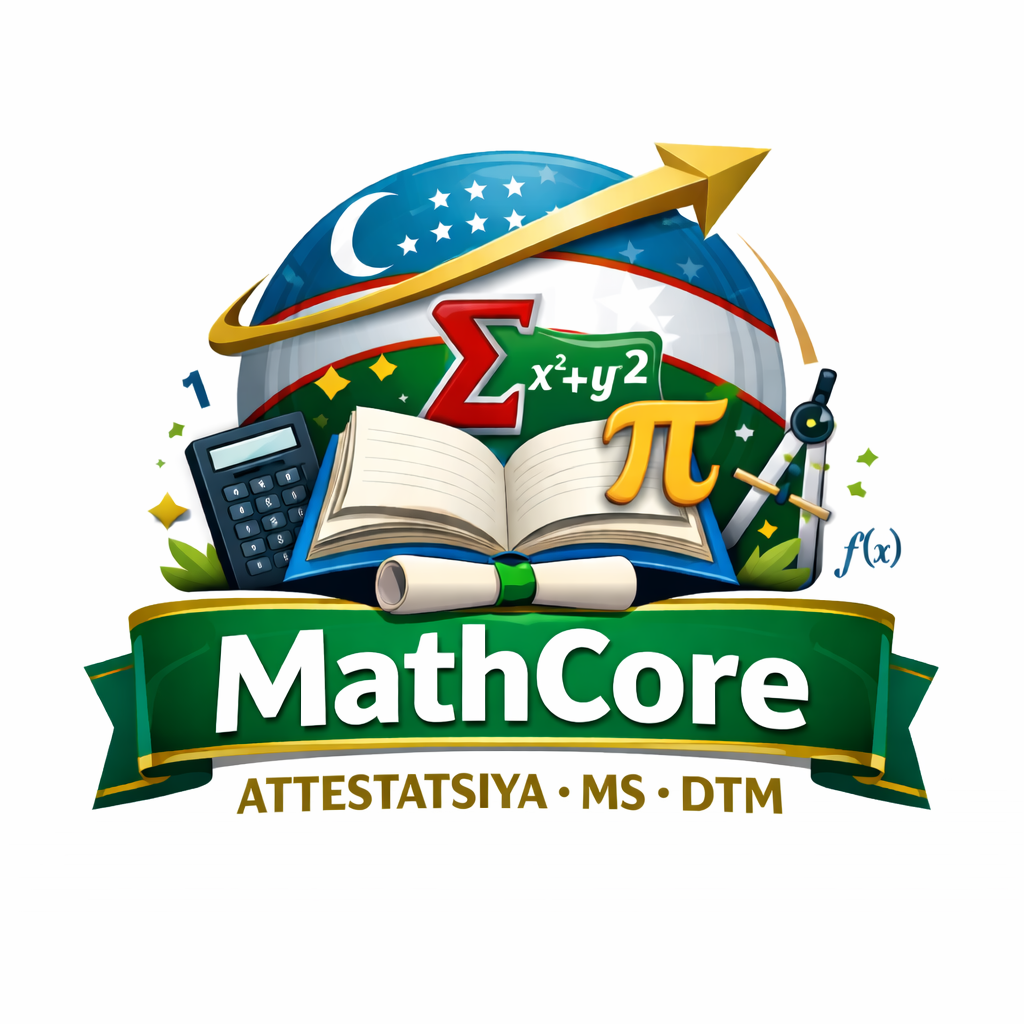
\includegraphics[width=0.2\textwidth]{logo.png} \\[5mm]
    \textcolor{gray}{\small Telegram: \href{https://t.me/Math_Core_Dtm_MS_Att}{@Math\_Core\_Dtm\_MS\_Att}}
\end{center}
\vspace{5mm}
% Задача 1
\begin{questionbox}{1}
    Определите, верны или неверны следующие утверждения:
    \begin{enumerate}
        \item[(I)] Если \(x_1, x_2, x_3\) — корни уравнения \(ax^3 + bx^2 + cx + d = 0\), то \(x_1 + x_2 + x_3 = -b/a\).
        \item[(II)] Уравнение окружности с центром \(O(a; b)\) и радиусом \(R\): \((x + a)^2 + (y + b)^2 \le R^2\).
        \item[(III)] Для производной сложной функции: \((g(f(x)))' = f'(x) g(f'(x))\).
    \end{enumerate}
    \begin{options}
        \item I – верно, II – неверно, III – неверно
        \item I – неверно, II – неверно, III – верно
        \item I – верно, II – верно, III – неверно
        \item I – неверно, II – верно, III – неверно
    \end{options}
\end{questionbox}

% Задача 2
\begin{questionbox}{2}
    Сколько простых чисел, меньших 2001, имеют сумму цифр, равную 2?
    \begin{options}
        \item 5
        \item 4
        \item 2
        \item 3
    \end{options}
\end{questionbox}

% Задача 3
\begin{questionbox}{3}
    В треугольнике \(ABC\) \(\angle B = \angle D\) (рис.), \(|AC| = 12\), \(|EC| = 4\) и \(S_{CDE} = 12\). Найдите \(S_{ABED}\).
\begin{dd}
        \centering
        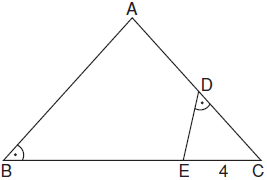
\includegraphics[width=0.5\linewidth]{eq.png}
    \end{dd}
        \begin{options}
        \item 108
        \item 48
        \item 98
        \item 96
    \end{options}
\end{questionbox}

% Задача 4
\begin{questionbox}{4}
    Натуральные числа от 1 до 1000 записаны подряд: 123...1000. Сколько раз в этой записи встречается цифра 7?
    \begin{options}
        \item 200
        \item 270
        \item 280
        \item 300
    \end{options}
\end{questionbox}

% Задача 5
\begin{questionbox}{5}
    Найдите остаток от деления \(7^3 + 11 \cdot 7\) на 6.
    \begin{options}
        \item 3
        \item 0
        \item 2
        \item 1
    \end{options}
\end{questionbox}

% Задача 6
\begin{questionbox}{6}
    Для натурального \(a\) выполнено \(a^2 - 1 = 8^7 (2^{19} + 1)\). Найдите \(\frac{a-1}{64^3}\).
    \begin{options}
        \item 16
        \item 4
        \item 8
        \item 32
    \end{options}
\end{questionbox}

% Задача 7
\begin{questionbox}{7}
    Окружность концентрична окружности \(x^2 + y^2 + 6x - 8y = 0\). Найдите уравнение касательной, проведённой из точки \(A(1; -3)\) к этой новой окружности.
    \begin{options}
        \item \(2x - 4y - 15 = 0\)
        \item \(4x - 2y + 23 = 0\)
        \item \(4x + 7y + 15 = 0\)
        \item \(4x - 7y - 25 = 0\)
    \end{options}
\end{questionbox}

% Задача 8
\begin{questionbox}{8}
    Дан многочлен \(P(x) = (x^2 - x + 2)^3\). Найдите \(d[P(x)] + P(1)\), где \(d[P(x)]\) — степень многочлена.
    \begin{options}
        \item 8
        \item 10
        \item 14
        \item 13
    \end{options}
\end{questionbox}

% Задача 9
\begin{questionbox}{9}
    Если \(\tg \alpha = -2\), найдите \(\frac{2\cos 2\alpha + 1}{1 - 3\cos^2 \alpha}\).
    \begin{options}
        \item \(-1{,}75\)
        \item \(-0{,}5\)
        \item \(-3{,}16\)
        \item \(-0{,}95\)
    \end{options}
\end{questionbox}

% Задача 10
\begin{questionbox}{10}
    Пусть \(m = (\sqrt{13} + \sqrt{11})^6\). Вычислите \(m \cdot (1 - \{m\})\), где \(\{a\}\) — дробная часть числа \(a\).
    \begin{options}
        \item 64
        \item 62
        \item 143
        \item 47
    \end{options}
\end{questionbox}

% Задача 11
\begin{questionbox}{11}
    Сколько положительных целых решений имеет неравенство \((x^2 - 1)\sqrt{6 - x - x^2} \le 0\)?
    \begin{options}
        \item 3
        \item 2
        \item 1
        \item 0
    \end{options}
\end{questionbox}

% Задача 12
\begin{questionbox}{12}
    Решите неравенство \(\sqrt[3]{x^{\log_3 \sqrt[3]{x} }} > 3\).
    \begin{options}
        \item \((1; +\infty)\)
        \item \((0; \frac{1}{27}) \cup (27; +\infty)\)
        \item \((0; 1)\)
        \item \(\varnothing\)
    \end{options}
\end{questionbox}

% Задача 13
\begin{questionbox}{13}
    Функция \(y = 8x + 19\) параллельно перенесена на вектор \(\mathbf{m}(6; 3)\). Найдите уравнение полученной функции.
    \begin{options}
        \item \(y = 8x - 26\)
        \item \(y = 8x - 29\)
        \item \(y = 8x - 23\)
        \item \(y = 8x + 23\)
    \end{options}
\end{questionbox}

% Задача 14
\begin{questionbox}{14}
    На рисунке изображены правильный треугольник и квадрат. Площадь их пересечения (закрашенной области) равна \(\frac{1}{6}\) площади треугольника и \(\frac{1}{4}\) площади квадрата. Найдите отношение стороны треугольника к стороне квадрата.
\begin{dd}
        \centering
        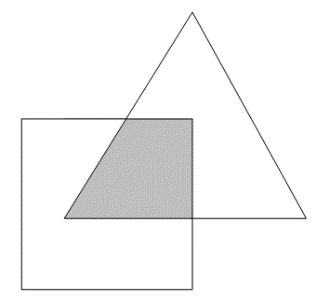
\includegraphics[width=0.3\linewidth]{rwt.png}
    \end{dd}
        \begin{options}
        \item \(2\sqrt[4]{3}\)
        \item \(2\sqrt{3}\) 
        \item \(\sqrt{2\sqrt{3}}\)
        \item 3
    \end{options}
\end{questionbox}

% Задача 15
\begin{questionbox}{15}
    Если \(3f(x) = f(x+1) + f(x-1)\), \(f(1)=3\), \(f(2)=4\), то сколько простых делителей имеет число \(f(5)\)?
    \begin{options}
        \item 6
        \item 1
        \item 3
        \item 2
    \end{options}
\end{questionbox}

% Задача 16
\begin{questionbox}{16}
    В уравнении \(\overline{abc} + \overline{cba} = 1453\) числа \(\overline{abc}\) и \(\overline{cba}\) — трёхзначные, \(a, b, c\) — цифры. Найдите \((a+c)\cdot b\).
    \begin{options}
        \item 64
        \item 80
        \item 45
        \item 91
    \end{options}
\end{questionbox}

% Задача 17
\begin{questionbox}{17}
    На пяти одинаковых карточках написаны буквы: О, Б, М, К, Р (без повторений). Карточки перемешивают и вынимают по одной. Найдите вероятность того, что в порядке извлечения получится слово «БОР».
    \begin{options}
        \item \(\frac{1}{60}\)
        \item \(\frac{1}{30}\)
        \item \(\frac{1}{40}\)
        \item \(\frac{1}{120}\)
    \end{options}
\end{questionbox}

% Задача 18
\begin{questionbox}{18}
    В треугольнике \(ABC\) (рис.) \(AD \perp BC\), \(AD\) — биссектриса, \(|BD| = |EC|\), \(\angle EBC = 20^\circ\). Найдите \(\angle BCA\).
\begin{dd}
        \centering
        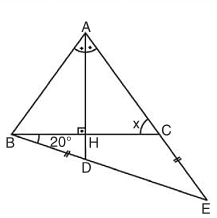
\includegraphics[width=0.3\linewidth]{wfg.png}
    \end{dd}
        \begin{options}
        \item \(45^\circ\)
        \item \(50^\circ\)
        \item \(55^\circ\)
        \item \(60^\circ\)
    \end{options}
\end{questionbox}

% Задача 19
\begin{questionbox}{19}
    На покраску металлического шара израсходовали 100 г краски. Сколько килограммов краски потребуется, если диаметр шара увеличить в 4 раза?
    \begin{options}
        \item 2,4 кг
        \item 3 кг
        \item 1,6 кг
        \item 1,8 кг
    \end{options}
\end{questionbox}

% Задача 20
\begin{questionbox}{20}
    Даны полуокружность и треугольник \(ABC\) с \(AB \perp AC\), \(BD = 3\), \(BE = 1\). Найдите \(FC : AF\).
\begin{dd}
        \centering
        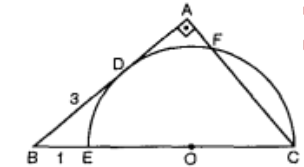
\includegraphics[width=0.5\linewidth]{hdjfj.png}
    \end{dd}
        \begin{options}
        \item 9
        \item 8
        \item 7
        \item 6
    \end{options}
\end{questionbox}

% Задача 21
\begin{questionbox}{21}
    Функция \(y = \ln^2 x - \ln x\) пересекает ось \(Ox\) в двух точках. Найдите площадь треугольника, образованного этими точками и точкой минимума графика функции.
    \begin{options}
        \item \(\frac{e^2 - 1}{2}\)
        \item \(\frac{e - 1}{4}\)
        \item \(\frac{e - 1}{8}\)
        \item \(\frac{e}{4}\)
    \end{options}
\end{questionbox}

% Задача 22
\begin{questionbox}{22}
    Вычислите: \(2\arctg\frac{1}{4} + \arctg\frac{7}{23}\).
    \begin{options}
        \item \(\frac{\pi}{4}\)
        \item \(\frac{3\pi}{4}\)
        \item \(\frac{\pi}{3}\)
        \item \(\frac{\pi}{6}\)
    \end{options}
\end{questionbox}

% Задача 23
\begin{questionbox}{23}
    Найдите произведение решений уравнения:
    \[
    y^2 + 2\sqrt{y^2 + 3y - 4} - 4 + 3y = 0.
    \]
    \begin{options}
        \item 4
        \item \(-1\)
        \item \(-4\)
        \item 1
    \end{options}
\end{questionbox}

% Задача 24
\begin{questionbox}{24}
    \(AB\) — диаметр, \(\angle ACE = 30^\circ\), \(\angle EDB = 40^\circ\). Найдите \(\angle ABD = \alpha\).
\begin{dd}
        \centering
        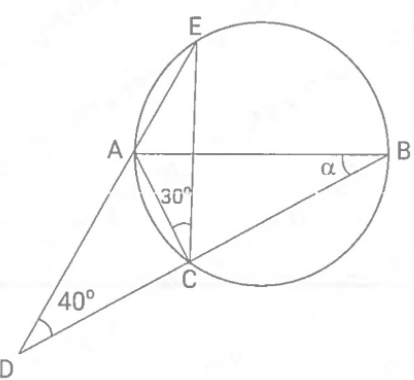
\includegraphics[width=0.3\linewidth]{thjh.png}
    \end{dd}
        \begin{options}
        \item \(15^\circ\)
        \item \(20^\circ\)
        \item \(25^\circ\)
        \item \(30^\circ\)
    \end{options}
\end{questionbox}

% Задача 25
\begin{questionbox}{25}
    Числа 5, 7, 11, 17, … таковы, что разности соседних членов образуют арифметическую прогрессию. Найдите 100-й член последовательности.
    \begin{options}
        \item 9605
        \item 9905
        \item 9745
        \item 10095
    \end{options}
\end{questionbox}

% Задача 26
\begin{questionbox}{26}
    Решите неравенство: \(4x \cdot \arccos(x^2 - 4x + 5) > x^2\).
    \begin{options}
        \item \(\{2\}\)
        \item \((1; 5)\)
        \item \((-2; 3)\)
        \item \(\varnothing\)
    \end{options}
\end{questionbox}

% Задача 27
\begin{questionbox}{27}
    Для треугольника выполнено равенство \(\frac{a}{\cos A} = \frac{b}{\cos B}\). Определите тип треугольника.
    \begin{options}
        \item правильный
        \item равнобедренный
        \item не существует
        \item тупоугольный
    \end{options}
\end{questionbox}

% Задача 28
\begin{questionbox}{28}
    \(ABCD\) — квадрат, \(EH \perp DF\), \(AE = EB = EH = 3\). Найдите \(BF/FC\).
\begin{dd}
        \centering
        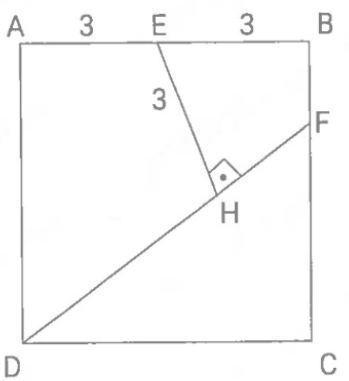
\includegraphics[width=0.3\linewidth]{gaa.png}
    \end{dd}
        \begin{options}
        \item \(\frac{1}{3}\)
        \item \(\frac{1}{2}\)
        \item \(\frac{2}{5}\)
        \item \(\frac{1}{4}\)
    \end{options}
\end{questionbox}

% Задача 29
\begin{questionbox}{29}
    Найдите сумму:
    \[
    1\cdot 3 + 3\cdot 3^2 + 5\cdot 3^3 + \dots + 93\cdot 3^{47}.
    \]
    \begin{options}
        \item \(47\cdot 3^{47} + 3\)
        \item \(46\cdot 3^{48} + 3\)
        \item \(48\cdot 3^{49} + 3\)
        \item \(46\cdot 3^{46} + 1\)
    \end{options}
\end{questionbox}

% Задача 30
\begin{questionbox}{30}
    Для последовательности \(a_0, a_1, a_2, \dots\) задано: \(a_0 = 1\) и \(a_{n+1} = 3a_n-a_{n-1}\). Найдите \(8a_1 -a_{3}\).
    \begin{options}
        \item 12
        \item 13
        \item 3
        \item 2
    \end{options}
\end{questionbox}

% Задача 31
\begin{questionbox}{31}
    Около окружности радиуса \(R=1\) описана равнобедренная трапеция площади 5. Найдите площадь четырёхугольника, вершины которого — точки касания окружности с трапецией.
    \begin{options}
        \item 1,6
        \item 1,7
        \item 1,8
        \item 1,9
    \end{options}
\end{questionbox}

% Задача 32
\begin{questionbox}{32}
    Для уравнения \(x^2 - (m+4)x + 2m + 5 = 0\) известно, что \(x_1 < 3 < x_2\). Найдите промежуток для \(m\).
    \begin{options}
        \item \((-2; 2)\)
        \item \((2; +\infty)\)
        \item \((-\infty; -2)\)
        \item \((-2; 0)\)
    \end{options}
\end{questionbox}

% Задача 33
\begin{questionbox}{33}
    Даны множества \(A = \{1,2,3,4,5,6,7\}\), \(B = \{1,2,4,5,7\}\), \(C = \{3,4,6,8\}\). Найдите \(A \setminus (B \cup C)\).
    \begin{options}
        \item \(\{8\}\)
        \item \(\{4\}\)
        \item \(\{4,8\}\)
        \item \(\varnothing\)
    \end{options}
\end{questionbox}

% Задача 34
\begin{questionbox}{34}
    В треугольнике \(ABC\) \(AD\) — биссектриса, \(AE\) — высота. Известно, что \(\angle ABC - \angle ACB = 28^\circ\). Найдите \(\angle DAE\) (в градусах).
    \begin{options}
        \item 13
        \item 14
        \item 15
        \item Неопределимо
    \end{options}
\end{questionbox}

% Задача 35
\begin{questionbox}{35}
    Даны точки \(A(0;12)\), \(C(6;0)\). Найдите \(S_{OBC}\) 
\begin{dd}
        \centering
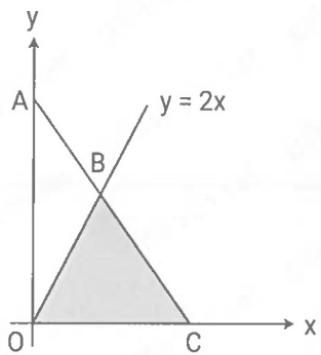
\includegraphics[width=0.3\linewidth]{daf2.png}
    \end{dd}
        \begin{options}
        \item 12
        \item 15
        \item 18
        \item 24
    \end{options}
\end{questionbox}

\end{document}